\chapter{Building India's Processor Ecosystem}

\centerline{{\large - An Interview With Prof. Kamakoti, IIT, Chennai}}

\vskip .5cm

\noindent\makebox[\textwidth]{\includegraphics[width=\textwidth]{src/Figures/authors/Kamakoti.jpg}}

\begin{multicols}{2}
Prof. Kamakoti of Indian Institute of Technology Madras is leading India's first successful attempt in developing a comprehensive range of processor families from tiny IoT class processors to server grade cores. Prof Kamakoti was awarded the ACCS-CDAC Foundation Award 2018 along with Prof Vijay Kumar of Indian Institute of Science. Prof. Kamakoti's dream of making an indigenous processor for India under Project Shakti, will reach critical milestone in April 2019 with the release of a server class chip using RISC V ISA. With this, IITM will be among the handful of institutions worldwide to have created a complete open source microprocessor ecosystem. ACCS writer, Prashanth Hebbar caught up with Prof. Kamakoti on his work. This is an excerpt from the interview.

{\bf Stanford, MIT and now IIT Madras have developed new processor ecosystems based on RISC V? Are we heading towards an industry which is more fragmented than ever? How do you characterize this new push towards RSIC V based processor ecosystems?}
\vskip 6pt

Today, when we look at the use of processors, there is a significant difference between what happened in the past and what is happening currently. One distinguishing mark between the previous century and this century is that the use of processors in different application domains has spread quite widely. Today, I use processors in washing machines, intelligent locks, surveillance cameras, agriculture, healthcare, physical fitness gadgets, public utility services, finance, POS machines, electronic voting machines and so on. I can keep on going.

The main issue here is heterogeneity. Today, if I talk just about IOT, the IOT that goes in a car is different from the IOT that goes in a smart glass. There is a lot of heterogeneity that comes up when you basically start looking at the kind of ways in which I am going to use technology. Which means, I may not be able to have one single processor [architecture] which may effectively and efficiently solve all the problems. That's why the 2018 Turing Award winners, John Hennessey and David Patterson, rightly said that you must look at domain specific [processor] architectures.

Customization of processors is the need of the day and open source will enable that customization and facilitate certain ecosystem which will make it economically viable.

{\bf In your paper on Shakti, you talked about the virtues of instruction set extensibility? Why is it important today?}

The domain specificity is what is going to be the success of this new era. The ability to add small hardware here and a small bit there to suit a particular use case, is facilitated by the instruction set architecture. So, extensibility of the instruction set architecture becomes crucial using which we can quickly add the extra instruction needed. We can also very quickly touch the software stack and make the compiler basically use new hardware we added. If the compiler doesn't use the system, then the hardware we added remains a waste.

{\bf That brings us to the questions of how efficient our compilers are? Do you see a problem there? How does RISC V and its extensible instruction set help here?}


Traditionally, there has been a big disconnect between compiler and the [processor] architecture. Take some of the old complex instruction set architectures which offer a lot of architectural features, but very rarely will the compiler even compile the code to [optimum levels] because compilers are fine tuned for a general impact.

The processor architecture companies have a huge compiler presence and they essentially fine tuning the compiler to a generalized impact but if someone attempts to fine tune further, they may not gain much -- usually 3-4\% gain is what achieved in such cases. I did my computer architecture assignment in 1992 under Professor Kalyan Krishnan (IIT Madras). We took a 32-bit C compiler to understand how much of the 32-bit features of the architecture is being used. We found out that only five percent of the total addressing words were being utilized and 95\% silicon was just lying there. This situation hasn't improved much in recent times.

These are some of the issues for effective functioning in special purpose hardware. If I am going to look at IOT where I have power restrictions, area restrictions, form factor, memory restrictions and so on, I need a lot of optimization.

In this context, RISC V ushers in an interesting paradigm. Let us take a simple example.  Today, many of the processors only set a flag when a divide by zero error occurs and do not automatically take you to an exception handler. That is handled by the compiler. Now, if you look at some of the safety critical applications, divide by zero is a nightmare and they must be handled right. Suppose, I need to make a processor for that type of safety critical application, using commercially off the shelf processors may just not be an answer. These kinds of issues are only the tip of the iceberg.

We are told that by 2022, there will be 50 billion IOT devices. Let us even say 10\% of it is true, that itself is a huge volume. Important to note is that these IOT devices are not gigahertz applications, they are megahertz applications and today many of these applications can even be run on an FPGA and structured ASIC. If you just take the FPGA and make a chip, it will be five times faster on one fifth the power.


{\bf What do you think is the tipping point of your work? What makes it different from other efforts across the world?}

For anyone to quickly make a processor and get it deployed is not easy. All said and done, with 12 students everything being new, we have been through two successful tape-outs. Both are running Linux, all the things that we wanted to port have been ported and it's working fine.

What stands out is that now we have an ecosystem wherein people can quickly take a processor, customize it to whatever their needs are, make applications, port their software, run it. All these things can be done on small Rs 5,000 FPGA boards. When satisfied, they can run volumes like in millions and can go for an ASIC. For smaller volumes, like 10,000 volumes, they make a smaller investment and make a structured ASIC and so on. 

This ecosystem now exists which is going to drive the real economic sense to what it means to make a processor.

{\bf What is the philosophy behind Shakti project, do you think it will be limited in scope because it's an academic project?}

\begin{figure}[H]
\centering
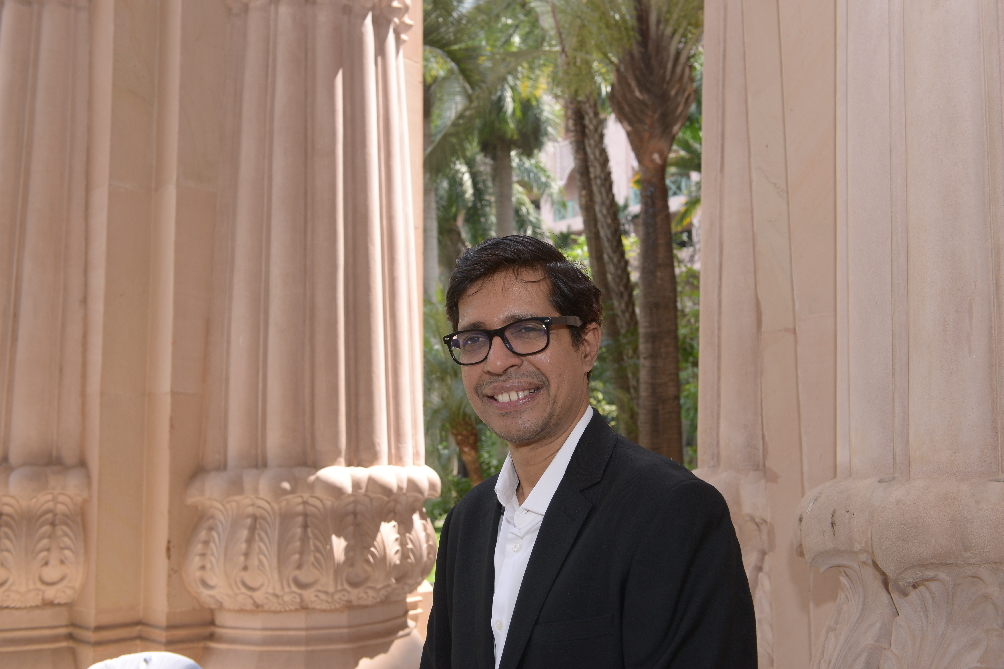
\includegraphics{src/Figures/authors/Kamakoti1.jpg}
\end{figure}
\vskip -0.6cm

As far as we are concerned at IIT Madras, all that we do are open source and we have made a conscious decision to release Shakti under BSD license which allows anyone to make anything including making profit from it and we will be happy. We are not looking at any revenue back from this. What we believe is that this will give our country the necessary technology.

We are doing it because we are an academic institute and we are in the juncture of a completely transforming digital world and at this point, we need to enable our country which is going to have a significant amount of electronic interference and manipulation; we need to enable our country with our designs which will make us feel comfortable. Comfort zone now comes with security.

Security is another point where you should forget completely about making money. There was a recent news article that an electronics-enabled vehicle could be hacked wherein when you press the break, it will accelerate and when you press the accelerator, it will break. With all these penetrations happening, we need to have a secure system. This whole project is trying to give open source environment where people can build boxes about which they know everything and there are absolutely no blind spots.
\smallskip

{\bf Are you looking at this from a security point of view alone like in a defense application or do you see Indian industry picking it up for civilian use? What applications is Shakti being put to?}

We are looking at this as a processor for India, both strategic and for civilian and consumer electronics. We did a survey and found around 493 different Indian companies who can potentially use Shakti. We have met around 20 of them and we will try and meet rest of them and see how they can benefit.

The companies we have met are in the consumer electronics application and security applications space and we also have certain strategic partners who have now come to us to build an ecosystem. There are a couple of startups, one from our own lab, who want to start building an ecosystem based on Shakti. We are helping them at the IIT level. We are also looking at a RedHat model, where startups can offer customization of the Shakti platform for a fee.

We have a 180-nanometer fab in Chandigarh that gave us a lot of confidence. We developed a processor and it worked in the first instance; the first tape-out was successful. We are also working on an open source CAD tool that is essential for security reasons or while designing for high performance.
\smallskip

{\bf What's your experience collaborating with other entities in this field and how much has Shakti gained from such collaborations? }

We are playing a significant role in a worldwide open source initiative called the ``Open Road Project''.  It was initiated by DARPA. We are now taking our design to make an open source tool flow for our SEL Fab, so any startup in India who wants to make a chip need not invest anything. They need not get scared about money or investment. I can sit in a garage and start working on it and then make a chip, like the open source software got made. We are democratizing the hardware and the tools. This will be the biggest success model for us.
\smallskip

{\bf What your motivation to start this project, how many man years did it take to achieve this level of accomplishment?}

We conceived this project around 2012-13 inspired by Dr. Abdul Kalam and our stated goal was to give India a commercially viable processor ecosystem by 2020. It's not just to make a processor, the goal was to make an ecosystem. If you don't have an ecosystem, then it will be another project where we will deliver and probably show proof of concept and it will live and die in some academic paper. 

We started off with Open Power but then it was not as open as we thought. Then RISC V started, we established a lot of contact with University of California, Berkeley. Rocket was the first chip made by Berkeley based on RISC V and then MIT came up with a chip.

In terms of architecture we are similar but what makes us different is that we need fault tolerance, security and intelligence. For fault tolerance we have tied up with Thallus. Thallus also came out with open source safety critical standards.  We are now building up the world class safety critical standards which will be out in a year and a half.  Thallus is funding that initiative under their open source funding.  So, we'll put out that work in open.

Security is not just putting crypto accelerators is not security, crypto is only 5\%; it's a very important thing, of course, as the entire route of trust depends upon crypto but in overall system building crypto is only playing a minor role although an important role. There are a lot of things that we need to do to handle in modern attacks like the SQL injection attacks and stuff like that so we are trying to build certain things in the spine of the microarchitecture. We have got a concept of tag destruction set architectures and we are giving lot more micro architectural aid to security. That will be our unique selling point. From an intelligence and security angle we don't we want to merely make it open we want to do the best and make it open.

Coming to intelligence, there are two parts to intelligence, one is intelligence at the edge and the intelligence at the server. We are working on both. There is a center sponsored by Kris Gopalakrishnan, our alumnus, Center for Computational Brain Research where we are working on neuromorphic brain inspired computing and we have made a lot of progress on that. We have given a proposal to MEITY to fund us the next stage. The entire project has been funded by MEITY and I should thank them for their trust in us. We also thank Intel who came out and did a free 22 nanometer tape-out for us in their semiconductor laboratory in Chandigarh and Synopsis and Hindustan Computers Ltd. have helped us too 

\section*{What's next in the Shakti paradigm?}

The next story for us is about supercomputing. We now have a very good grip over multicores. We have a framework where we can make N number of cores theoretically. We want to look at this as 32 to 64 core single-chip and we are also working with standards such as the Interconnect. This is going to be a single SOC yielding something like 2.5 gigahertz per core easily. We call it ParaShakti which means Parallel Shakti. 

As of today, we have the understanding and the ability to roll out an FPGA level prototype of ParaShakti, it just costs a million dollars.


\noindent
{\bf Finally, do you think your project can really be the precursor to an Indian processor ecosystem?}


  Of course, that has been our mission. I call it as India's project. Some scientists at MEITY say it's `your proposal' and I say, `no this is our proposal'. I want to push that very clearly. From an academic point of view, we must do something constructive for the country. We know that there is a problem and we know God has given us the brains to solve that problem; we can't keep quiet and that is the prime motivation for us. Beyond that as a country we need to solve this issue of security, indigenous development, democratizing hardware, democratizing software infrastructure and thus as a country in the national security perspective, nothing in the country should not stop because of lack of technology.\raisebox{-.1cm}{
\includegraphics[scale=.9]{src/Figures/circledC.eps}}

\begin{center}

\includegraphics{src/Figures/An_Interview_QR.png}
\medskip

{\large Access this article on the Web}
\end{center}
\end{multicols}
\medskip


